
\documentclass[brazilian,12pt,a4paper,final]{article}


\usepackage[a4paper,
bindingoffset=0.2in,
left=0.8in,
right=0.8in,
top=0.8in,
bottom=0.8in,
footskip=.25in]{geometry}

%% Pacotes extras (opcionais):

% *babel* contem as regras de hifenização
\usepackage[portuguese]{babel}
% *t1enc* permite o reconhecimento dos acentos inseridos com o teclado
\usepackage{t1enc}

% *inputenc* com opção *utf8* permite reconhecimento dos caracteres com codificação UTF8, que é padrão dos esditores de texto no Linux. Isso permite reconhecimento automático de acentuação.
%\usepackage[utf8]{inputenc}
\usepackage{epsfig}

% *graphicx* é para incluir figuras em formato eps 
\usepackage{graphicx} % para produzir PDF diretamente reescrever esta linha assim: \usepackage[pdftex]{graphicx}

% *color* fontes soloridas
\usepackage{color}
%%% fim do cabecalho %%%

\pagestyle{empty}
\title{Métodos Computacionais Aplicados à Biocomplexidade}
\author{Aluno: André Gustavo Dessoy Hubner - Matrícula: 00315569 \\ IF-UFRGS}

\begin{document}
	\maketitle
	
	\section{Introdu\c{c}\~ao} 
	% Aqui a Introdução \c{c} e \~a  é a forma standar  de escrever
	% carateres ASCII extendidos (acentos, etc), porem com o pacote t1enc
	% declarado acima podemos escrever diretamente ç em lugar d \c{c}, etc
	\indent 
	Este documento trata de um programa experimental para a identificação de genes de proteína, rRNA e tRNA em genomas
	bacterianos criado através de Python.
	Aqui será exposto o racional por traś da metodologia usada, assim como diversos outros pontos que
	elucidam a utilidade de ferramentas desse tipo para a resolução de problemas da Biotecnologia
	envolvendo anotação de genomas.
	
	\section{Metodologia}
	\subsection{Busca de genes convencionais}
	\subsubsection{Classe Genome, configuração e inicialização}
	Primeiramente, foi criada uma classe chamada de \textit{Genome}, que é usada para conter informações
	importantes e levá-las aos diversos métodos da anotação de genoma, que também estão contidos nela. No
	método construtor desta classe (\_\_\_init\_\_\_), foram definidos seis parâmetros cujos valores passados 
	pelo usuário configurarão todo o funcionamento da anotação para a instância gerada. A partir da instância
	da classe Genome, então, basta rodar o método AnnotateGenome, que chamará todas os métodos envolvendo 
	o processo da anotação de genoma. Chamar métodos outros que este ocasionará em erro, uma vez que estão todos 
	marcados como métodos privados ou protegidos justamente para que não haja funções sendo processadas em ordem errada. A única
	exceção é o método SearchRNAGenes, que pode ser chamado sozinho para realizar a busca apenas por genes de
	RNA.
	
	\vspace{0.5cm}
	
	Dos seis parâmetros supracitados, apenas um é obrigatório, sendo este o primeiro, em que é especificado o caminho
	do sistema de onde buscar o arquivo .fasta contendo a sequência do genoma a ser analisado. Devido ao projeto ser
	experimental, outros tipos de entrada resultarão em erro. A sequência do arquivo será então utilizada pelo método
	GetSequence, através de manipulação de arquivo e string básica de Python, para extrair apenas a sequência, sem as informações
	contidas na primeira linha, e armazená-la como um membro de instância. Os cinco parâmetros opcionais, por sua vez, tem funções 
	conforme a seguinte tabela:
	
	\vspace{0.5cm}
		
	\begin{itemize}
		\item minProb: produto mínimo das probabilidades dos Boxes -10 e -35 em relação ao possível gene (ponto
						que será explicado em uma seção posterior), de forma que ele seja
						considerado como um gene candidato. Assim, é possível controlar o equilíbrio quantidade/qualidade
						dos candidatos utilizando este parâmetro. Padrão 0 (sem filtro).
						
		\item minSize: semelhantemente ao caso acima, controla a qualidade dos genes candidatos, porém filtrando-os pelo
						tamanho da sua sequência codificadora. Padrão 3 (tamanho do códon de início).
						
		\item includeRNAGenes : booleano que indica se serão buscados genes não só de DNA como de RNA também no método 
								AnnotateGenome. como todos os 3 parâmetros posteriores também estão envolvidos na busca
								de genes de RNA, se este parâmetro tiver o valor de "False", os três não terão nenhum efeito.
								Padrão False.
		\item  searchString : string que deve corresponder a um organismo o qual será utilizado para obter as sequências padrão
								de rRNA e tRNA para a busca dos mesmos na sequência de genoma da instância. A obtenção dessas 
								sequências padrão é uma funcionalidade experimental e é realizada por busca no banco de dados do NCBI
								, ocasionando um aumento significativo do tempo de processamento. No entanto, uma vez que se sabe que as sequências de tRNA e rRNA entre bacterias pode variar bastante, a utilização de uma searchString tendo como alvo o organismo correto pode trazer um impacto bastante positivo na busca. Caso não seja especificada nenhuma string
								ou passada uma string vazia assim como por padrão, serão utilizadas sequências locais de Escherichia coli sem 
								realizar a busca por API, demandando assim muito menos tempo de processamento. 
								Padrão string vazia.							    
		\item rnaGenesMinScore inteiro usado como score mínimo de um gene de RNA para ser considerado como candidato, permitindo controlar a abordagem quantidade/qualidade para genes de RNA também. Padrão 0.
	\end{itemize}
								
	
		A figura 1 mostra um exemplo de instanciação da classe Genome, realizando logo após a anotação da sequência especificada buscando por genes de proteínas 
		de tamanho mínimo de 3, produto das probabilidades de no mínimo 0.25, e genes de RNA com intervalo entre cada gene de no mínimo 30 nucleotídeos, com 
		score mínimo de 0,25 também e usando os padrões locais de Escherichia coli, conforme especificado no construtor da classe. Como já está implícito,
		A possibilidade de configurar a pesquisa com diferentes parâmetros permite fazer buscas com diferentes configurações facilmente.
		
		\vspace{0.5cm}
		
		O último ponto desta parte de configuração envolve a obtenção da sequência reversa da obtida no arquivo para obter também os genes possíveis
		 neste lado da fita de DNA. Isto é feito já no método AnnotateGenome, utilizando um dicionário contendo os reversos de cada nucleotídeo para obter uma
		 tabela de tradução, e então, após "virar" a sequência padrão com fatiamento de strings, usando esta tabela para convertê-la na sequência reversa. Devido ao caráter experimental do projeto, a busca na fita
		 reversa só foi considerada para genes de proteínas.
		 
		
	\begin{figure}[hbtp]
		\begin{center}
			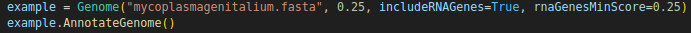
\includegraphics[]{../Figures/Instanciacao.png}
			\caption{figura demonstrando a criação de uma instância da classe Genome e a realização da anotação do genoma por ela}
			\label{fig}
		\end{center}
	\end{figure}

		\subsubsection{Métodos essenciais na busca por genes de proteína}
	Para iniciar a busca de genes de produtos alvos de tradução em dada sequência foi construído o método GetGene, que recebe a sequência alvo e um número n, buscando os genes a partir da
	n-ésima posição na sequência (considerando indexação baseada em 0). O ponto essencial dessa busca é que ela utiliza o método find de strings para, a partir de n,
	na sequência como string, buscar uma substring igual a "ATG". Achado o primeiro ATG a partir de n, ocorrerá uma iteração de 3 em 3 nucleotídeos na sequência até achar um 
	códon de parada, parando então a busca e retornando o índice de início e o de fim do gene candidato. Caso não seja encontrado um ATG a partir de n, o valor retornado
	é -1, que é captado dentro do método para significar que a busca por genes  acabou na sequência. Um ponto importante a considerar neste método foi que, devido
	ao genoma bacteriano ser circular, é possível que um gene comece perto da extremidade final do genoma (pelo menos considerando a representação em arquivo .fasta) e termine
	na extremidade de início ou até adiante. Para representar este ponto foi adicionado mais um laço de repetição no código, impedindo que um gene perto da extremidade final da string seja cortado devido a ter chegado no "fim" da sequência.
	
	\vspace{0.5cm}
	
	Em seguida, atentando-se que em genes de bacterias existem duas regiões muito importantes para a transcrição da sequência, conhecidos como TATA boxes -10 e -35 (justamente por estarem a posições de -10 e -35 nucleotídeos em relação ao início da sequência codificadora), chamados de agora em diante de boxes 10 e 35, foi construído um método para dar uma pontuação a uma certa sequencia de entrada
	para avaliá-la como um TATA box dependendo da sequência consenso do TATA box, que também é informada por entrada (parâmetro). O esquema de pontuação utilizado envolve, tendo como base um valor de 1, iterar por toda a sequência e, se o caractere atual for igual ao do consenso, multiplicar a pontuação pela porcentagem condizente ao nucleotídeo consenso naquela posição; caso contrário, a multiplicação ocorre com a probabilidade de não ser aquele nucleotídeo (\((1-p)/3\), considerando p como a probabilidade de ser o nucleotídeo consenso)	pela sequência em questão.
	
	\vspace{0.5cm}
	
	Tanto GetGenes quanto GetPontuation são pontos fundamentais do programa, sendo executados iterativamente pelos métodos explicados na próxima subseção e tendo suas lógicas fundamentais aplicadas semelhantemente para a busca de genes de RNA. A figura 2 mostra o funcionamento do primeiro método, enquanto que a figura 3 faz o mesmo para o segundo.
	
	\begin{figure}[hbtp]
		\begin{center}
			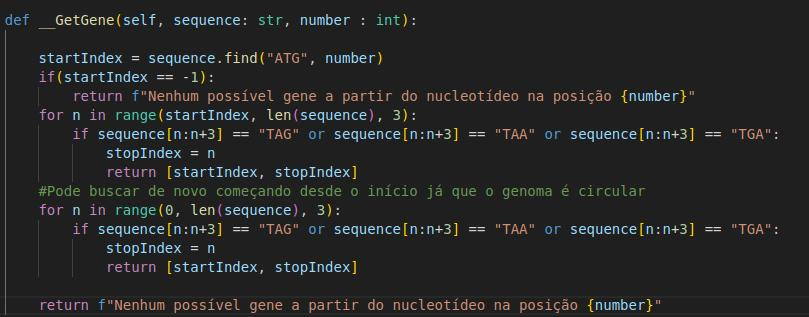
\includegraphics[width=15cm]{../Figures/GetGene.jpg}
			\caption{Busca da sequência codificadora de um possível gene, dado um genoma alvo e um número para começar a buscar, pelo método GetGene.}
			\label{fig}
		\end{center}
	\end{figure}

\begin{figure}[hbtp]
	\begin{center}
		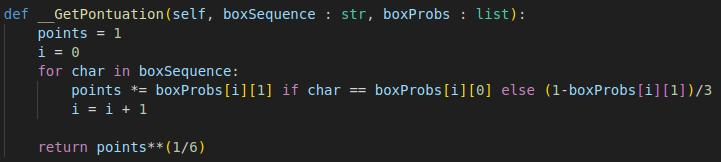
\includegraphics[width=15cm]{../Figures/GetPontuation.jpg}
		\caption{Atribuição da pontuação de uma sequência como TATA box para o padrão de box espećificado em boxProbs. boxProbs também deve conter as probabilidades associadas com cada nucleotídeo consenso, permitindo o cálculo da pontuação.}
		\label{fig}
	\end{center}
\end{figure}

\subsubsection{Busca iterativa de genes candidatos}
Dados os métodos construídos anteriormente, era necessário juntá-los em algo que percorresse o genoma inteiro. Primeiro, considerando um possível gene já achado, construiu-se o método GetBestBoxes que, recebendo um genoma e o a posição de início do gene achado neste genoma, retorna os boxes 10 e 35 de maior pontuação para o gene associado. Este passo é necessário uma vez que os TATA box não estão necessariamente a exatamente 10 e 35 nucleotídeos a montante do codon de início. Na verdade, sabe-se que a distância entre o início e primeiro box pode ser de 6 a 10 nucleotídeos, enquanto que o outro box pode estar de 17 a 20 nucleotídeos de distância do box -10. Logo, a função deste método é justamente de buscar qual sequência de 6 nucleotídeos entre todas nessas posições tem a melhor pontuação para o respectivo TATA box, utilizando o método GetPontuation como descrito anteriormente. A implementação foi bastante condizente com a descrição acima, conforme demonstrado na figura 4. O método retorna uma lista contendo as pontuações dos melhores boxes 10 e 35, além de uma string representando todos os nucleotídeos do códon de início até o box -35, com uma representação logo abaixo dos melhores boxes identificados da respectiva sequência consenso utilizada.

\begin{figure}[hbtp]
	\begin{center}
		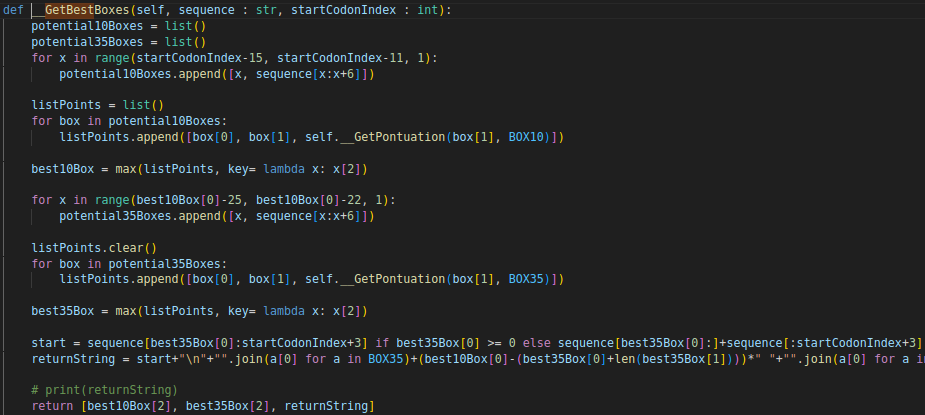
\includegraphics[]{../Figures/GetBestBoxes.png}
		\caption{Método GetBestBoxes, que vasculha a região a montante do gene candidato encontrado, retornando as pontuações dos melhores boxes encontrados assim como uma representação em string da região. Código parcialmente cortado devido ao tamanho}
		\label{fig}
	\end{center}
\end{figure}
	
	
	\vspace{0.5cm}
Finalmente, o método FindGenes representou a junção de todas as peças desse quebra-cabeça. Recebendo o genoma alvo como string e uma lista onde serão armazenados os resultados, sua função é garantir a busca iterativa por genes no genoma especificado até que se chegue ao fim. No código isso ocorre dentro de um laço While com o argumento "True", especificando portanto que a iteração ocorra até que algo a impeça explicitamente. Logicamente o primeiro método a ser chamado é o GetGene, começando a busca pela posição 0, e então apenas se esse gene tiver o tamanho mínimo parametrizado na inicialização da instância se buscará pelos melhores boxes com GetBestBoxes. Por fim, se o produto das probabilidades dos boxes encontrado nesta última chamada for maior que probabilidade mínima dos parâmetros, adiciona-se esse gene, incluindo informações relevantes retornadas pelos métodos anteriores na lista para retorno. Independentemente de se o gene atual cumpriu as restrições dos parâmetros a busca por genes começa novamente a partir da posição de início deste gene, fluindo normalmente até que GetGene retorne uma string representando o fim da busca, que será identificada pela função nativa isInstance, quebrando o laço While e retornando a lista com as informações dos genes identificados. Este método está representado na figura 5.

\vspace{0.5cm}

\begin{figure}[hbtp]
	\begin{center}
		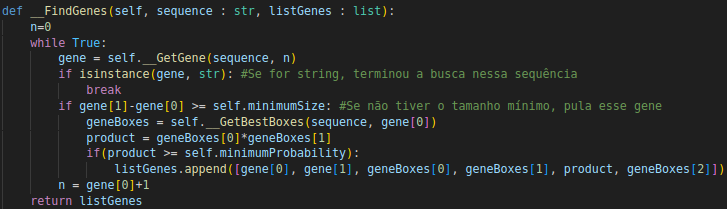
\includegraphics[]{../Figures/FindGenes.png}
		\caption{Iteração por todo o genoma pesquisando por genes candidatos e retornando seus dados pelo método FindGenes}
		\label{fig}
	\end{center}
\end{figure}

Uma vez achados todos os genes possíveis para a fita padrão do arquivo do genoma, o mesmo processo se repetirá tendo como base o outro lado da fita, usando a sequência obtida através da tabela de tradução assim como descrito no fim da primeira subseção, e adicionando os novos candidatos à mesma lista de retorno.
Finalizada a busca por genes de proteína, se iniciará em seguida a busca por genes de rRNA e de tRNA caso o usuário tenha passado includeRNAGenes como True.

\subsection{Busca de genes de rRNA e tRNA}
\subsubsection{Obtenção dos padrões e buscas no NCBI}
Contextualizando a solução para a busca de genes de rRNA e tRNA, ela teve um caráter experimental e considerou abordagens que poderiam ser utilizadas para resolver o problema a mão, especialmente conhecimentos difundidos sobre esses tipos de genes. Isso é visto logo de início, pois antes de iniciar a busca por esses genes, pode-se buscar os padrões de 16S rRNA, 5S rRNA e 23S rRNA e de todos os tRNAs para o organismo específicado em "searchString", de forma a melhorar a qualidade dos resultados obtidos. 

\vspace{0.5cm}

Mais detalhadamente, essa busca ocorre nos métodos "GetrRNATemplate" e "GettRNAsTemplates", onde ocorre a busca pela sequência em questão de forma  semelhante, acessando a conexão ao Entrez do Biopython, primeiro com uma função "esearch" onde se procura pelos resultados de uma pesquisa como se fosse feita na página do NCBI, tendo o banco de dados "nucleotide" como alvo e abrindo os resultados desejados através da função "efetch".

\vspace{0.5cm}

No entanto, as duas abordagens utilizadas variam da mesma forma que a disponibilidade dessas sequências variam no banco de dados. A primeira função é chamada três vezes, uma vez para buscar cada rRNA de forma que as strings de busca utilizadas mudem conforme o caso. Como existia a possibilidade de serem retornados dados substancialmente diferentes dos desejados, foi necessária bastante meticulosidade na elaboração da busca. Por fim, essa busca é realizada garantindo que o resultado contenha palavras como rRNA, gene, o nome deste rRNA e um tamanho de sequência próximo daquele conhecido para rRNAs do tipo em questão, optando por aqueles com tamanhos mais próximos.
\\
\vspace{0.5cm}

A busca de padrões de rRNA, por sua vez, teve que levar em conta a escassez dessas sequências como resultados separados no NCBI. Contornando essa limitação, programou-se a execução de "esearch" neste contexto mirando em genomas do organismo possuindo features a respeito de genes de tRNA e excluindo potenciais sequências incompletas do resultado. Adicionalmente se buscou pelos detalhes desses resultados com "esummary" de forma a poder obter o resultado mais atual, selecionando ele com "efetch" e convertendo sua representação para um formato Genbank que no passo seguinte  (método \_\_ExtracttRNASequence) permite a extração da sequência de gene de tRNA para cada aminoácido no campo de features do genoma. As sequências obtidas são então armazenadas se tiverem um tamanho de entre 100 e 65 nucleotídeos, próximo dos cerca de 78 nucleotídeos que é o tamanho estipulado médio para genes de tRNA.

\vspace{0.5cm}

Apesar da influência positiva esperada nos resultados devido ao aproveitamento dessas sequências personalizadas, é bastante notável o aumento do tempo de execução do programa advindo da busca delas. Mesmo após paralelizar o processamento das 4 chamadas responsáveis, passo antes do qual demorava cerca de 30 segundos para buscar todos os padrões, esse tempo varia perto dos 9 segundos, aproximadamente 5 vezes o tempo para buscar genes de proteína. Portanto, a utilização do parâmetro "searchString" deve ser criteriosa. Terminada esta etapa, a busca por genes de RNA poderá começar através de AnnotateGenome após a fase de genes de proteína, ou chamando SearchRNAGenes que realizará unicamente a busca por genes de RNA.

\vspace{0.5cm}

\subsubsection{Busca por genes de rRNA e tRNA}
\vspace{0.5cm}

A partir de SearchRNAGenes as buscas por genes de rRNA e tRNA serão feitas de forma paralela nos métodos SearchrRNAGenes e SearchtRNAGenes, respectivamente,  tendo uma lógica similar à utilizada para genes de proteína, com a principal diferença, contudo, na forma como a pontuação (score) é calculada. Para genes candidatos de tRNA e de rRNA, seu score será calculado comparando cada nucleotídeo desde um ponto igual em 3 nucleotídeos ao padrão, adicionando 1 a uma soma caso sejam iguais. Essa comparação ocorrerá para o mesmo número de nucleotídeos do tamanho da sequência padrão, dividindo então por este e obtendo portanto a proporção de nucleotídeos que ambas as sequências têm em igual. Os resultados retornados para os dois tipos de RNA estão no formato [posição inicial, fim, score].

\vspace{0.5cm}


No primeiro método, para cada rRNA a ter candidatos buscados, será criado um laço de repetição While marcado com True que chama um método para buscar um gene, parando a busca caso seja retornada uma string e adicionando o produto aos resultados caso ele tenha uma pontuação maior à do filtro que, neste caso, é o determinado pelo parâmetro rnaGenesMinScore. Após o fim dessa busca, representada pelo método \_\_rRNAGenesIterations, poderá ser feita mais uma volta pelo genoma buscando pelos genes caso o resultado dessa busca anterior esteja vazio.

\vspace{0.5cm}

 Decidiu-se por essa implementação pois muitas vezes os padrões achados na fase anterior possuem nucleotídeos não convencionais marcados com "N" que impossibilitam encontrar qualquer resultado. Nesses casos então a primeira volta pelo genoma termina na primeira chamada ao método de buscar gene, e logo após será realizada uma volta efetiva de busca substituindo esse nucleotídeo por uma adenosina para pelo menos ter resultados. Esse processo inteiro também foi paralelizado com o intuito de executar para cada tipo de rRNA paralelamente, salvando quase 10 segundos do tempo de iteração.
 
 \vspace{0.5cm}
 
 Concorrentemente, a busca por genes de tRNA ocorrerá de forma semelhante, sendo as iterações performadas dentro do método \_SingletRNASearch que é chamado para todos os aminoácidos, atribuindo seus resultados a um dicionário contendo os aminoácidos com chaves e os as listas das informações dos genes como valores. Ambas as buscas retornarão resultados como string "sem resultados" caso não encontrem resultados para o tipo em questão, permitindo assim que análises sejam feitas com certos tipos de genes de RNA mesmo que não tenha sido possível obter outros tipos.
 
 \vspace{0.5cm}
 
 Aqui ambas as buscas rodam por cerca de 18 segundos em uma busca padrão, logo com a paralelização de ambas foi possível resguardar uma boa quantidade de tempo. Terminadas ambas as buscas, também termina SearchRNAGenes e logo depois AnnotateGenome, sendo todos os resultados durante a execução de cada método podendo ser obtidos por retorno direto ou chamando o respectivo membro de instância após a finalização.
 Com os todas as funcionalidades implementadas, bastava analisar os resultados


\begin{figure}[hbtp]
	\begin{center}
		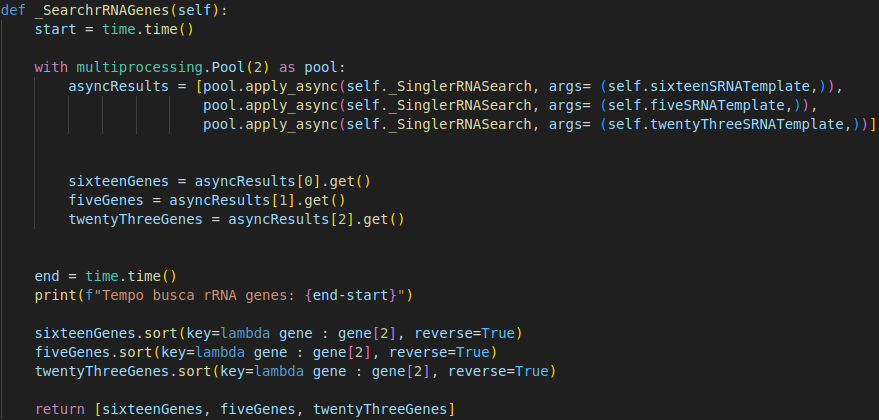
\includegraphics[width=15cm]{../Figures/SearchrRNAGenes.png}
		\caption{Busca por genes de rRNA 16S, 5S e 23S, iterando pelo genoma ao menos uma vez para cada caso. Aqui as chamadas a SinglerRNASearch representam cada uma dessas buscas, performando uma lógica semelhante à usada para genes de proteína}
		\label{fig}
	\end{center}
\end{figure}

\begin{figure}[hbtp]
	\begin{center}
		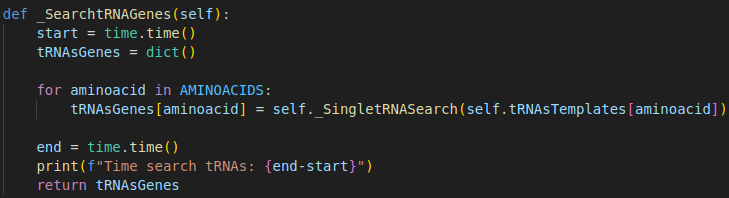
\includegraphics[width=15cm]{../Figures/SearchtRNAGenes.png}
		\caption{Busca por todos os genes de tRNA, iterando uma vez pelo genoma para cada tRNA a ser buscado. Semelhamente, aqui SingletRNASearch está encarregado de cada um desses casos.}
		\label{fig}
	\end{center}
\end{figure}	
	
	\section{Resultados}
	\vspace{0.5cm}
	\subsection{Testando filtros de tamanho de CDS e probabilidade e dados gerais }
	Para as análises estatísticas envolvendo gráficos utilizou-se a biblioteca Matplotlib de Python, que já é bem estabelecida para análises deste perfil, em um arquivo separado chamado de "Análises estatísticas.py". Almejou-se medir o impacto do filtro de tamanho de CDS no número e qualidade dos possíveis genes de proteína obtidos na anotação de genoma, aproveitando para isso a chamada de AnnotateGenome em diferentes instâncias de Genome, tendo portanto os seus resultados disponíveis para fornecer como input nas funções de construção de gráfico em figuras do Matplotlib. 
	
	 \vspace{0.5cm}
	
	Para a primeira figura, foram comparados dados de oito instâncias com diferentes filtros mínimos de tamanho de CDS. Dessas, a primeira atuava sem filtro, a segunda com tamanho mínimo de 30, a terceira de 100, a quarta de 300 e a partir de então cada instância tinha um filtro maior em 300 nucleotídeos até a última instância com tamanho mínimo de 1500 nucleotídeos.
	Tendo como pontos do eixo x o tamanho mínimo de cada instância e no eixo y o número de genes para cada um deles, plotou-se então um gráfico de barras, que pode ser observado na figura 8.
	
	\begin{figure}[hbtp]
		\begin{center}
			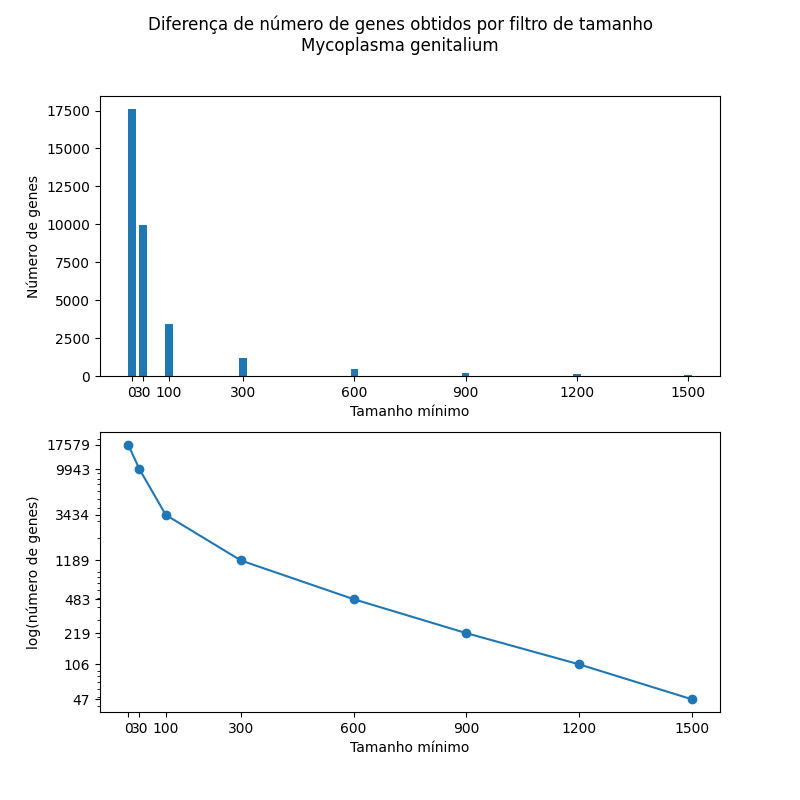
\includegraphics[width=15cm]{../Figures/FiltroTamanho.png}
			\caption{Figura contendo dados sobre o número de genes para cada busca com diferentes filtros tamanho mínimo de CDS. O segundo gráfico está em escala logarítmica no eixo y, ajudando a ver os valores exatos para cada ponto do eixo x}
			\label{fig}
		\end{center}
	\end{figure}
	
	
	 \vspace{0.5cm}
	
	Como é possível observar, de forma pouco surpreendente, filtros de tamanhos mínimos menores obteram bem mais genes candidatos, ao ponto que é difícil apontar um valor aproximado aos genes obtidos para as instâncias de filtros maiores. Por esse motivo, realizou-se outra plotagem, desta vez configurando o eixo y de forma que esteja em escala logarítmica e seus pontos marcados em cada valor exato de y, além de colocar retas ligando cada ponto. Com isso, obteve-se o segundo gráfico na figura 8, que além dos números exatos de genes para cada filtro demonstra também uma tendência de redução dos genes semelhante a um padrão logarítimico conforme se aumenta o tamanho de CDS mínimo de acordo com os valores usados.
	
	 \vspace{0.5cm}
	
	Ainda para essas instâncias, calculou-se a média dos boxes de cada gene de cada instância, imprimindo-os ao terminal ao rodar esse arquivo. Nesses dados, observa-se que a distribuição das médias varia muito pouco, sendo as maiores e menores médias do box10 de 0.2577 (27,77\%) e 0.2502 (25,02\%), e do box35 de 0.2431 (24,31\%) e 0.2328(23,28\%), respectivamente, outro fato esperado, uma vez que a diferença do tamanho dos CDS não deveria afetar significativamente a qualidade dos candidatos obtidos.
	
	 \vspace{0.5cm}
	
	Já o próximo gráfico teve como objetivo verificar a funcionalidade do filtro de produto mínimo entre as probabilidades dos boxes 10 e 35, aproveitando também para saber a quantidade de genes para cada probabilidade que são retornados. Para isso, foram utilizados histogramas em que o eixo x representa uma faixa de probabilidades do box 10 ou 35, enquanto que o eixo y representa o número de genes encontrados para essa probabilidade nesse box. Para este estudo, foram escolhidas três instâncias : a primeira sendo sem filtro; a segunda com produto mínimo de 15\%, representando um filtro intermediário; e o terceiro com produto mínimo de 25\%, filtrando a maioria dos genes. Plotou-se portanto 6 gráficos, todos representados na figura 9.
	
	\begin{figure}[hbtp]
		\begin{center}
			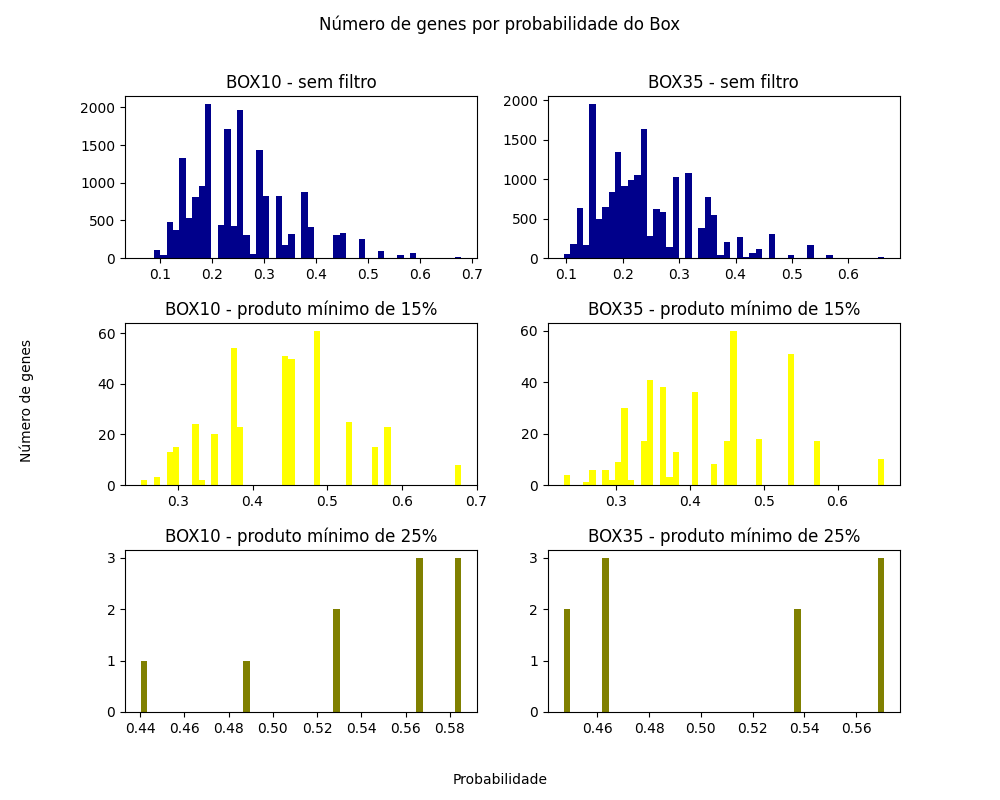
\includegraphics[width=15cm]{../Figures/FiltroPorcentagem.png}
			\caption{Histogramas representando o número de genes por valor de probabilidade para o BOX10 na primeira coluna e para o BOX35 na segunda, comparando os resultados por linha, que representam dados das buscas sem filtro, produto mínimo 15\% e produto mínimo 25\%, respectivamente. São bastante perceptíveis a diminuição no número de genes e o ajustamento dos scores encontrados à valores maiores conforme se aumenta a rigidez do filtro}
			\label{fig}
		\end{center}
	\end{figure}
	
	 \vspace{0.5cm}
	
	O primeira inferência clara que se pode a fazer a partir do resultado é que filtros de valores maiores reduzem drasticamente a quantidade de resultados, sendo observados apenas 10 genes para o filtro de 25\%, ao passo que sem filtro são obtidos 17579 genes (visualizável na figura 8). A segunda é que, sem filtro, parece haver uma proeminência muito grande de genes com probabilidades dos boxes até 40\%, enquanto que nos gráficos dos filtros essa probabilidade parece estar em valores significativamente acima, com cerca de metade dos genes identificados estando em probabilidades acima de 40\% usando o filtro de 15\% e todos estando acima dessa faixa para o filtro de 25\%. De fato, de acordo esses dados, usar valores maiores no parâmetro de produto de probabilidades mínimo aparenta ser uma forma eficiente de controlar rigidamente o equilíbrio entre qualidade e quantidade dos produtos a serem obtidos.
	
	 \vspace{0.5cm}
	
	Feita essa última análise, percebeu-se que ainda não se havia visualizado o número de genes obtidos por tamanho. Portanto, nesta etapa foi gerado um gráfico para visualizar justamente isso, aproveitando também para observar as diferenças nessas estatísticas entre os casos sem filtro, com tamanho mínimo de 600 e tamanho mínimo de 1500. Essa visualização está disponível novamente em formato de histograma, de acordo com a figura 10. Além disso, realizou-se o cálculo do tamanho médio de cada uma dessas instâncias, obtendo os valores de aproximadamente 91, 990 e 1945, seguindo a ordem anterior e denotando novamente o efeito esperado ao usar esse tipo de filtro. Com isso, foram finalizadas as análises para genes de proteína.
	
	\begin{figure}[hbtp]
		\begin{center}
			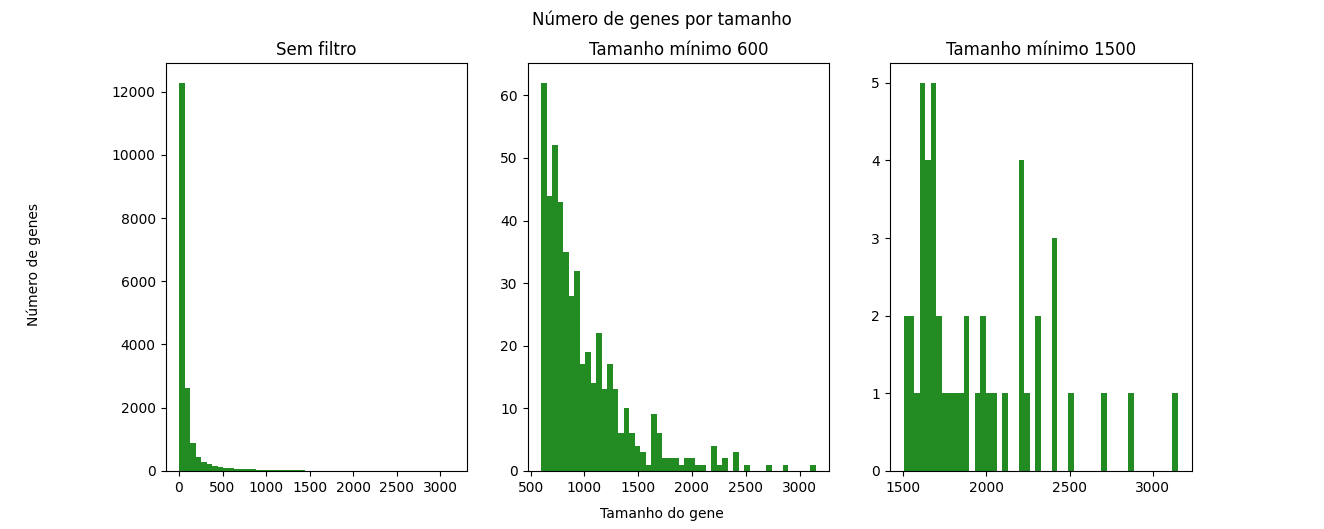
\includegraphics[width=15cm]{../Figures/GenesPerSize.png}
			\caption{Histogramas das buscas sem filtro, tamanho mínimo 600 e tamanho mínimo 1500, representando cada uma o número de genes obtidos para cada tamanho. Observa-se uma diminuição extrema do número de genes e o funcionamento correto do filtro de tamanho mínimo}
			\label{fig}
		\end{center}
	\end{figure}
	
	 \vspace{0.5cm}
	
	\subsection{Resultados de rRNA, tRNA e do filtro de score de RNAs}
	 \vspace{0.5cm}
	A última seção, por sua parte, teve como intuito validar a abordagem utilizada na busca por genes de rRNA e tRNA no que tange o número de genes encontrados e o score deles, levando em conta o papel do uso de sequências padrão do organismo alvo no resultado obtido. Para isso, tanto para genes de rRNA quanto de tRNA, foram usadas três instâncias: a primeira percorrendo os métodos de RNA de forma padrão, apenas com o parâmetro "includeRNAGenes" assinalado; a segunda contendo adicionalmente o parâmetro "rnaGenesMinScore" com o valor 0.25; e a terceira baseando-se na primeira, porém buscando sequências de \textit{Mycoplasma genitalium} para usar como padrão.
	
	 \vspace{0.5cm}
	
	A primeira  e a segunda figura foram bem simples: com base nos resultados de genes de cada rRNA nessas instâncias, fez-se histogramas plotando a quantidade de genes por scores de cada rRNA mostrado na figura 11. Assim, visualizando por colunas, é possível perceber que na primeira a distribuição é muito semelhante a uma gaussiana, enquanto que a segunda coluna parece representar a metade de maior pontuação do gráfico imediatamente à esquerda, percebendo-se então o funcionamento do parâmetro de score mínimo. Se aproveitou a mesma estratégia para construir uma figura equivalente para os resultados de três tRNAs (alanina, glutamina e treonina como exemplo) nessas duas instâncias, obtendo de novo esse padrão, como é possível ver na figura 12.
	
	\begin{figure}[hbtp]
		\begin{center}
			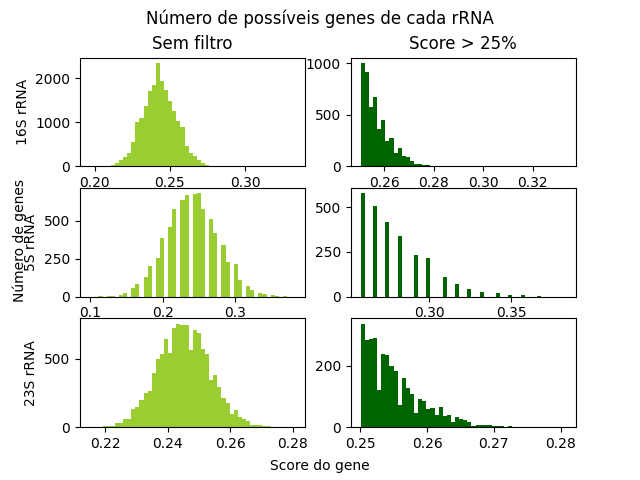
\includegraphics[width=15cm]{../Figures/genesrRNA.png}
			\caption{Distribuição de número de genes por score dos resultados de rRNA com ou sem o filtro de valor mínimo de 25\%.}
			\label{fig}
		\end{center}
	\end{figure}

\begin{figure}[hbtp]
	\begin{center}
		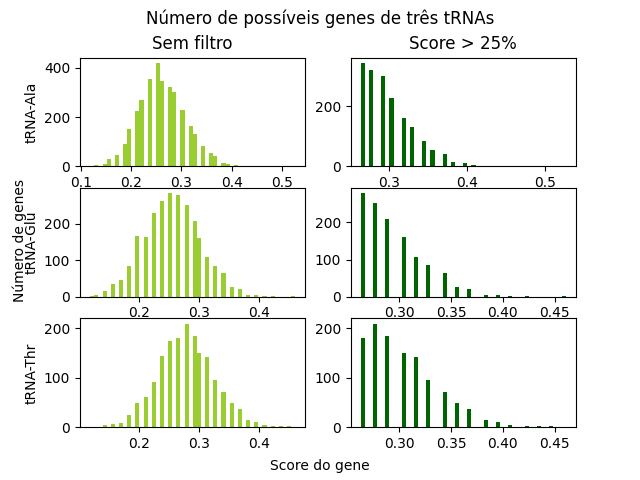
\includegraphics[width=15cm]{../Figures/genestRNA.png}
		\caption{Distribuição de número de genes por score dos resultados de tRNA com ou sem o filtro de valor mínimo de 25 \%}
		\label{fig}
	\end{center}
\end{figure}	
	
	 \vspace{0.5cm}
	
	 Por outro lado, partindo da curiosa semelhança dos histogramas da primeira coluna a uma distribuição normal, poderia-se suspeitar da eficiência da abordagem aplicada aqui. Isso, contudo, não é nada fora do comum e realmente esperado, uma vez que o genoma analisado neste projeto é da bacteria \textit{Mycoplasma genitalium}, cujo gênero é bastante idiossincrático, conhecido por ter vários dos organismos com os menores genomas conhecidos e possuindo padrões de metabolismo bastante diferentes devido a essa limitação. Logo, sem dúvidas é um organismo bastante diferente de \textit{Escherichia coli}, organismo cujos genes de tRNA e rRNA são usados como padrão para obter o score caso não haja "input" no parâmetro "searchString", sendo razoável esperar um resultado não significativo para casos em que o organismo do genoma a ser avaliado é substancialmente diferente daquele cujos padrões serão utilizados.
	 
	  \vspace{0.5cm}
	 
	
	Inspirando-se nessa questão, a próxima análise teve como objetivo visualizar as diferenças dos resultados de RNA usando uma instância com busca convencional e outra com sequências do NCBI. A primeira estratégia adotada aqui foi de utilizar histogramas da mesma forma que na primeira coluna das últimas duas figuras, porém agora para as duas buscas, tanto para os resultados de rRNA quanto de tRNA, estando elas disponíveis nas figuras 13 e 14.
	
	 \vspace{0.5cm}

	\begin{figure}[hbtp]
		\begin{center}
			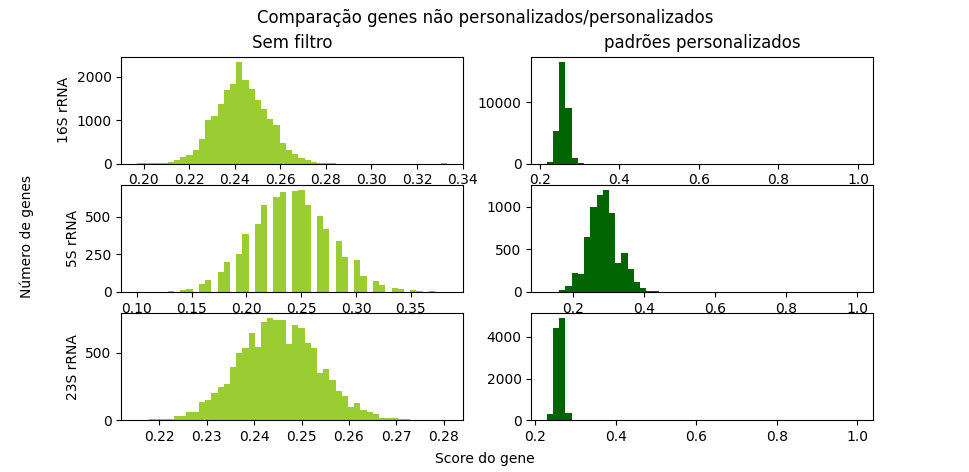
\includegraphics[width=15cm]{../Figures/PersonalizadosrRNA.png}
			\caption{Histogramas confrontando buscas com sequências armazenadas localmente e buscas com sequências do organismo alvo encontradas no NCBI para rRNAs, aplicando o mesmo padrão da primeira coluna dos casos anteriores para ambas as instâncias. Nota-se um aparente leve aumento da média de scores para os rRNAs 16S e 5S, porém o resultado de 23S é difícil de visualizar. Também se percebe que o gráfico de todos vai até o final devido à presença da sequência exata do padrão encontrado no NCBI }
			\label{fig}
		\end{center}
	\end{figure}
	
	\begin{figure}[hbtp]
		\begin{center}
			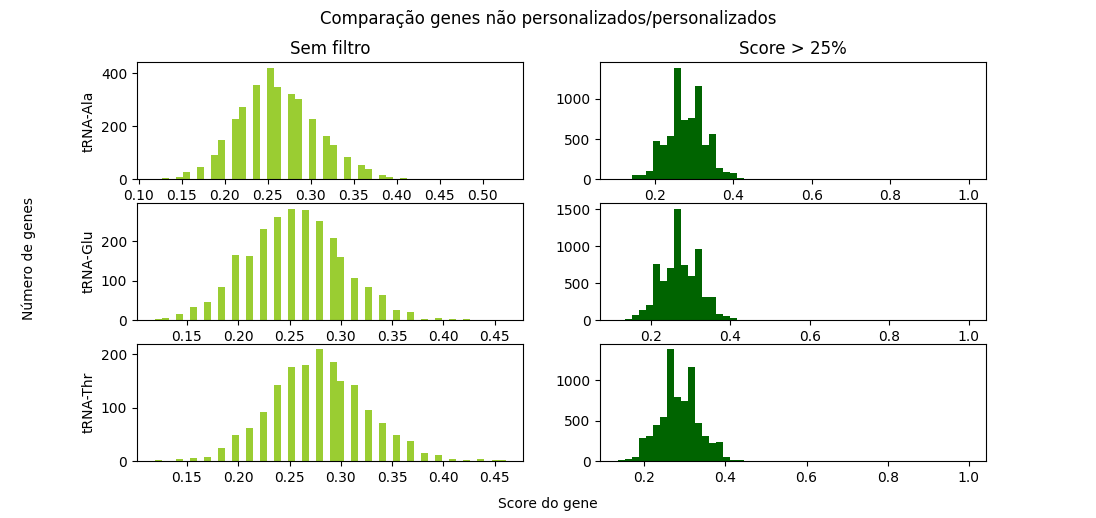
\includegraphics[width=15cm]{../Figures/PersonalizadostRNA.png}
			\caption{Semelhantemente à última figura, mostra de número de genes por score, desta vez para três casos de tRNA. Aqui a melhora nos scores é pouco perceptível e também se encontra a extensão até o score de 1 nos gráficos devido à sequência exata ter sido encontrada.}
			\label{fig}
		\end{center}
	\end{figure}

	Tanto para o cenário dos rRNAs quanto para os tRNAs, olhando meramente para a densidade dos pontos as melhoras foram leves no máximo. Contudo, a extensão de todos os gráficos construídos significa que foram encontrados resultados exatamente iguais ao padrão obtido na busca especificando \textit{Mycoplasma genitalium}" em "searchString", logo a identificação de genes utilizando esta ferramenta encontraria pelo menos esses genes. Este fato valida o funcionamento correto de da busca por genes de RNA.
	
	\vspace{0.5cm}
	
	Por outro lado, se sentia que a amostragem visual não era o suficiente até então, sendo construídos novos gráficos mostrando essa distribuição no formato stripplot da biblioteca Seaman nas figuras 15 e 16. Felizmente, a marcação de pontos deste tipo de gráfico proprorcionou não só o descobrimento dos resultados idênticos em rRNAs e tRNAs, como também de scores mais significativos especialmente para os genes candidatos de tRNA-Thr e tRNA-Ala que seria impossível de visualizar anteriormente e que podem ser sequências de herança evolutiva com o gene de tRNA encontrado no mesmo gŕafico.
	
	\vspace{0.5cm}
	
	Assim, sabendo-se que \textit{Mycoplasma genitalium} possuí apenas uma cópia dos rRNAs buscados, poucas cópias de genes de tRNAs também e foram encontrados resultados com score 1 em todos os tRNAs, possivelmente encontrando todos os genes de RNA de \textit{Mycoplasma genitalium}, essa abordagem de busca de RNAs foi um sucesso para o seu objetivo aqui. A última análise performada teve como objetivo identificar se a média dos scores dos genes de RNA das figuras acima aumentou mesmo retirando os resultados idênticos, que aqui funcionam como "outliers", procurando ver concretamente se esta abordagem ajudaria a encontrar produtos de parentesco evolutivo com as sequências buscadas. As médias para cada caso estão expostas seguindo a tabela 1.
	
	
	\begin{table*}[b]
		\centering
		\begin{tabular}{lcr}
				& busca convencional & busca personalizada \\
			16S & 0.2429 & 0.2597 \\
			5S & 0.2408 & 0.2849 \\
			23S & 0.2451 & 0.2601 \\
			Ala-tRNA & 0.2617 & 0.2796 \\
			Glu-tRNA & 0.2558 & 0.2697 \\
			Thr-tRNA & 0.2785 & 0.3676 \\
		\end{tabular}
		\caption{Comparação da média dos scores dos genes de RNA entre busca convencional e busca com o parâmetro "searchString" aplicado corretamente.}
		\label{tab:1}
	\end{table*}

	\begin{figure}[hbtp]
		\begin{center}
			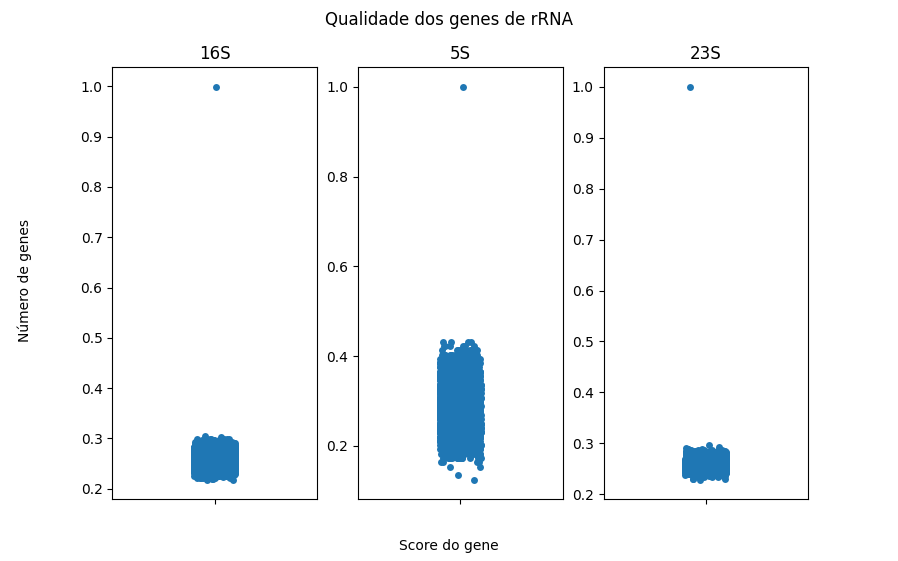
\includegraphics[width=15cm]{../Figures/DistribuiçãorRNA.png}
			\caption{Mostra novamente a distribuição dos resultados de cada rRNA para a busca com o padrão de \textit{Mycoplasma genitalium}, porém possibilitando visualizar agora as cópias idênticas encontradas.}
			\label{fig}
		\end{center}
	\end{figure}

	\begin{figure}[hbtp]
		\begin{center}
			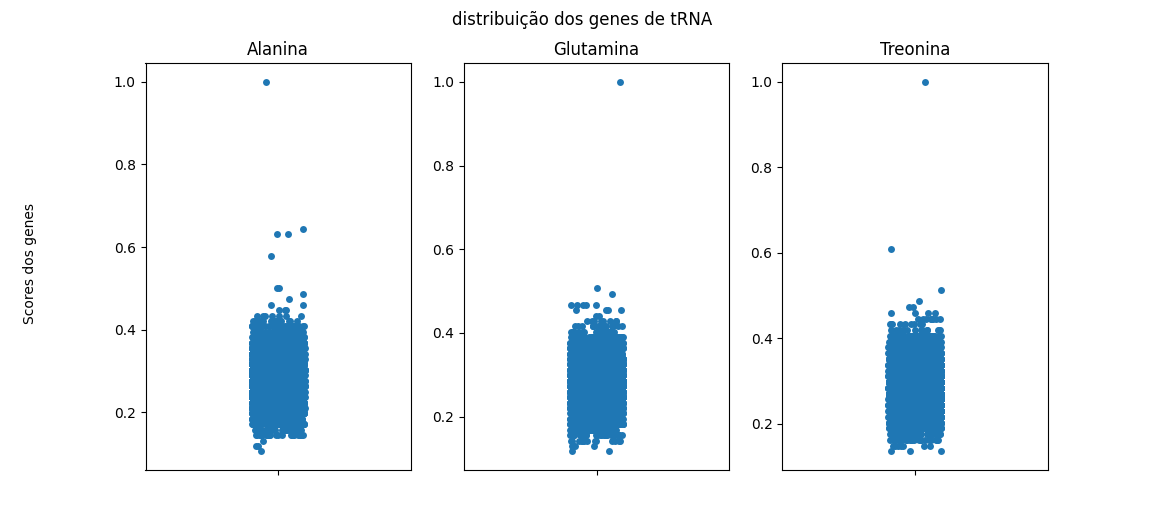
\includegraphics[width=15cm]{../Figures/DistribuiçãotRNA.png}
			\caption{Mostra novamente a distribuição dos resultados de cada tRNA para a busca com o padrão de \textit{Mycoplasma genitalium}, porém possibilitando visualizar agora as cópias idênticas encontradas e alguns resultados mais significativos que passariam despercebidos na metodologia anterior.}
			\label{fig}
		\end{center}
	\end{figure}

	
	\section{Considerações finais}
	Foi possível, portanto, encontrar resultados interessantes e validar os algoritmos de busca tanto no caso de genes de proteína quanto para genes de RNA. Para os genes que são traduzidos, utilizar o controle de produto das probabilidades mínimo e tamanho mínimo ajudou a focar os resultados em possíveis genes com valores para estes atributos bem mais altos. Um exemplo disso é que considerando um produto mínimo de 15\%, foi possível obter cerca de 300 genes tendo as pontuações de cada box de 30\% para cima, um número bastante significativo tendo em conta os cerca de 470 genes codificadores de proteína de \textit{Mycoplasma genitalium}.
	
	\vspace{0.5cm}
	
	Já para as buscas de genes de rRNA e tRNA, não só foi possível obter resultados significativos como possivelmente, utilizando o organismo alvo em "searchString", todos os genes de RNA deste organismo, além de algumas sequências de putativo parentesco evolutivo, dados os altos scores. Evidentemente os resultados não seriam tão significativos caso o genoma alvo fosse em um organismo possuindo mais cópias de genes de RNA, uma vez que na implementação atual só é possível buscar uma sequência para servir de padrão para cada gene de RNA. Por outro lado, isso seria apenas uma escalabilização do processo atual, não devendo ser algo tão complicado.
	
	\vspace{0.5cm}
	
	Finalmente, este projeto cumpriu seu objetivo, apresentando no processo alternativas claras para melhorar ainda mais os resultados, incluindo sistemas de pontuação mais refinados, possibilidade de usar mais conhecimentos sobre o organismo e o armazenamento de mais padrões como mencinado acima. 
	
	
	
\end{document}

